
%% bare_jrnl.tex
%% V1.4b
%% 2015/08/26
%% by Michael Shell
%% see http://www.michaelshell.org/
%% for current contact information.
%%
%% This is a skeleton file demonstrating the use of IEEEtran.cls
%% (requires IEEEtran.cls version 1.8b or later) with an IEEE
%% journal paper.
%%
%% Support sites:
%% http://www.michaelshell.org/tex/ieeetran/
%% http://www.ctan.org/pkg/ieeetran
%% and
%% http://www.ieee.org/

%%*************************************************************************
%% Legal Notice:
%% This code is offered as-is without any warranty either expressed or
%% implied; without even the implied warranty of MERCHANTABILITY or
%% FITNESS FOR A PARTICULAR PURPOSE! 
%% User assumes all risk.
%% In no event shall the IEEE or any contributor to this code be liable for
%% any damages or losses, including, but not limited to, incidental,
%% consequential, or any other damages, resulting from the use or misuse
%% of any information contained here.
%%
%% All comments are the opinions of their respective authors and are not
%% necessarily endorsed by the IEEE.
%%
%% This work is distributed under the LaTeX Project Public License (LPPL)
%% ( http://www.latex-project.org/ ) version 1.3, and may be freely used,
%% distributed and modified. A copy of the LPPL, version 1.3, is included
%% in the base LaTeX documentation of all distributions of LaTeX released
%% 2003/12/01 or later.
%% Retain all contribution notices and credits.
%% ** Modified files should be clearly indicated as such, including  **
%% ** renaming them and changing author support contact information. **
%%*************************************************************************


% *** Authors should verify (and, if needed, correct) their LaTeX system  ***
% *** with the testflow diagnostic prior to trusting their LaTeX platform ***
% *** with production work. The IEEE's font choices and paper sizes can   ***
% *** trigger bugs that do not appear when using other class files.       ***                          ***
% The testflow support page is at:
% http://www.michaelshell.org/tex/testflow/



\documentclass[journal]{IEEEtran}
%
% If IEEEtran.cls has not been installed into the LaTeX system files,
% manually specify the path to it like:
% \documentclass[journal]{../sty/IEEEtran}

\usepackage{xeCJK} % CJK语言环境,使用XeLaTex进行编译
\usepackage{authblk} % 对应中文部分的作者机构特殊语法
\usepackage{graphicx}
\usepackage{caption2}

% 将 authblk 包中的作者连词 and 替换为中文逗号
\renewcommand*{\Authsep}{,}
\renewcommand*{\Authand}{,}
\renewcommand*{\Authands}{,}

% *** GRAPHICS RELATED PACKAGES ***
%
\ifCLASSINFOpdf
  % \usepackage[pdftex]{graphicx}
  % declare the path(s) where your graphic files are
  % \graphicspath{{../pdf/}{../jpeg/}}
  % and their extensions so you won't have to specify these with
  % every instance of \includegraphics
  % \DeclareGraphicsExtensions{.pdf,.jpeg,.png}
\else
  % or other class option (dvipsone, dvipdf, if not using dvips). graphicx
  % will default to the driver specified in the system graphics.cfg if no
  % driver is specified.
  % \usepackage[dvips]{graphicx}
  % declare the path(s) where your graphic files are
  % \graphicspath{{../eps/}}
  % and their extensions so you won't have to specify these with
  % every instance of \includegraphics
  % \DeclareGraphicsExtensions{.eps}
\fi
% graphicx was written by David Carlisle and Sebastian Rahtz. It is
% required if you want graphics, photos, etc. graphicx.sty is already
% installed on most LaTeX systems. The latest version and documentation
% can be obtained at: 
% http://www.ctan.org/pkg/graphicx
% Another good source of documentation is "Using Imported Graphics in
% LaTeX2e" by Keith Reckdahl which can be found at:
% http://www.ctan.org/pkg/epslatex
%
% latex, and pdflatex in dvi mode, support graphics in encapsulated
% postscript (.eps) format. pdflatex in pdf mode supports graphics
% in .pdf, .jpeg, .png and .mps (metapost) formats. Users should ensure
% that all non-photo figures use a vector format (.eps, .pdf, .mps) and
% not a bitmapped formats (.jpeg, .png). The IEEE frowns on bitmapped formats
% which can result in "jaggedy"/blurry rendering of lines and letters as
% well as large increases in file sizes.
%
% You can find documentation about the pdfTeX application at:
% http://www.tug.org/applications/pdftex




% correct bad hyphenation here
\hyphenation{op-tical net-works semi-conduc-tor}


\begin{document}
%
% paper title
% Titles are generally capitalized except for words such as a, an, and, as,
% at, but, by, for, in, nor, of, on, or, the, to and up, which are usually
% not capitalized unless they are the first or last word of the title.
% Linebreaks \\ can be used within to get better formatting as desired.
% Do not put math or special symbols in the title.
\title{基于YOLOv8的头盔检测模型\\设计与实现}
%
%
% author names and IEEE memberships
% note positions of commas and nonbreaking spaces ( ~ ) LaTeX will not break
% a structure at a ~ so this keeps an author's name from being broken across
% two lines.
% use \thanks{} to gain access to the first footnote area
% a separate \thanks must be used for each paragraph as LaTeX2e's \thanks
% was not built to handle multiple paragraphs
%

\author{陈邵杰,郭昊,蔡明珠,刘政,黄俊毅,王晶昊,杨双菁,田睿朴,苗馨月% <-this % stops a space
\thanks{感谢电子科技大学机器学习课程闫老师与张老师的教学。}% <-this % stops a space
\thanks{2024年10月}}

% note the % following the last \IEEEmembership and also \thanks - 
% these prevent an unwanted space from occurring between the last author name
% and the end of the author line. i.e., if you had this:
% 
% \author{....lastname \thanks{...} \thanks{...} }
%                     ^------------^------------^----Do not want these spaces!
%
% a space would be appended to the last name and could cause every name on that
% line to be shifted left slightly. This is one of those "LaTeX things". For
% instance, "\textbf{A} \textbf{B}" will typeset as "A B" not "AB". To get
% "AB" then you have to do: "\textbf{A}\textbf{B}"
% \thanks is no different in this regard, so shield the last } of each \thanks
% that ends a line with a % and do not let a space in before the next \thanks.
% Spaces after \IEEEmembership other than the last one are OK (and needed) as
% you are supposed to have spaces between the names. For what it is worth,
% this is a minor point as most people would not even notice if the said evil
% space somehow managed to creep in.



% The paper headers
\markboth{Journal of \LaTeX\ Class Files,~Vol.~14, No.~8, October~2015}%
{Shell \MakeLowercase{\textit{et al.}}: 机器学习课程设计报告}
% The only time the second header will appear is for the odd numbered pages
% after the title page when using the twoside option.
% 
% *** Note that you probably will NOT want to include the author's ***
% *** name in the headers of peer review papers.                   ***
% You can use \ifCLASSOPTIONpeerreview for conditional compilation here if
% you desire.




% If you want to put a publisher's ID mark on the page you can do it like
% this:
%\IEEEpubid{0000--0000/00\$00.00~\copyright~2015 IEEE}
% Remember, if you use this you must call \IEEEpubidadjcol in the second
% column for its text to clear the IEEEpubid mark.



% use for special paper notices
%\IEEEspecialpapernotice{(Invited Paper)}




% make the title area
\maketitle

% As a general rule, do not put math, special symbols or citations
% in the abstract or keywords.
\begin{abstract}
随着人工智能的发展和交通安全需求的增加,基于深度学习的目标检测技术在行人头盔佩戴检测中发挥着重要用。在本研究中,针对行人检测场景采用YOLOv8l模型进行头盔检测,并通过稀疏化和剪枝技术对模型进行优化,在高精度的同时提升推理效率。利用稀疏化方法对YOLOv8l模型的权重进行优化,增强模型的稀疏性,减少计算冗余。通过剪枝技术有效去除冗余的网络参数和连接,大幅减少模型的计算量和参数规模,优化后的模型在嵌入式和边缘计算设备上运行效率显著提升。实验结果表明,经过稀疏化和剪枝后的YOLOv8l模型参数量减少了约30\%,推理速度提高了近40\%,并且在行人头盔检测任务中维持了高达98\%的准确率。我们还将优化后的模型与YOLOv3、YOLOv5、YOLOv7等多个版本进行了对比,验证了YOLOv8l在行人检测精度和速度方面的优势。
\end{abstract}

% Note that keywords are not normally used for peerreview papers.
\begin{IEEEkeywords}
交通管理,YOLOv8,头盔检测,深度学习,识别
\end{IEEEkeywords}

% For peer review papers, you can put extra information on the cover
% page as needed:
% \ifCLASSOPTIONpeerreview
% \begin{center} \bfseries EDICS Category: 3-BBND \end{center}
% \fi
%
% For peerreview papers, this IEEEtran command inserts a page break and
% creates the second title. It will be ignored for other modes.
\IEEEpeerreviewmaketitle

%1 引言
\section{引言}

%1.1课题背景及意义
\subsection{选题背景与意义}
Subsection text here.
%1.1.1课题背景
\subsubsection{课题背景}
subsubsection text here.
%1.1.1研究意义
\subsubsection{研究意义}
subsubsection text here.

%1.2研究问题分析
\subsection{研究问题分析}
Subsection text here.

%2 引言
\section{行人数据图像处理}
The conclusion goes here.

%2.1 实验数据集
\subsection{实验数据集}
Subsection text here.A'
%2.2 图像预处理
\subsection{图像预处理}
Subsection text here.
%2.3 yolo标准数据集
\subsection{yolo标准数据集}
Subsection text here.
%2.4 数据集标注
\subsection{数据集标注}
Subsection text here.

%3 基于YOLOv8的检测系统实现
\section{基于YOLOv8的检测系统实现}
The conclusion goes here.
%3.1 训练环境搭建
\subsection{训练环境搭建}
Subsection text here.

%3.2 模型训练
\subsection{模型训练}
Subsection text here.

%3.3 模型部署
\subsection{模型部署}
Subsection text here.

%4 调整与改进
\section{调整与改进}
电动自行车头盔的检测可能由于骑手的高速移动或环境的复杂性而变得颇具挑战性。例如,头盔可能因与摄像头距离较远而成为难以辨识的小目标。针对检测过程中低分辨率图像及小目标检测困难,背景与检测目标相似等问题,改进Yolov8n 模型。传统目标检测网络容易忽略或误判电动车骑行过程中远处、边缘或比例较小的头盔,进而导致漏检或误检。对此需要增强原始YOLOv8n模型以提升对小目标检测精度。
%4.1 
\subsection{卷积注意力模块}
本研究采用了基于卷积注意力机制模块\cite{ref1}(Convolutional Block Attention Module, CBAM)的小目标检测优化策略。CBAM作为一种即插即用的注意力机制模块,可直接嵌入至多种流行的卷积神经网络架构中。该模块通过对输入特征图的不同区域赋予不同的权重,使网络能够更加聚焦于对特定任务具有重要性的信息,同时忽略不相关的信息。因此,在针对佩戴头盔的行人检测任务中,由于目标与摄像头距离较远导致行人及头盔尺寸较小,且在检测图像中所占比例较低,引入CBAM能够使网络更加专注于前景中的小目标,并有效定位感兴趣的区域。这进一步增强了网络的特征提取能力,使得在最小感受野的特征图上能够更精确地识别小目标。CBAM的总体架构如图\Ref{fig:CBAM}所示。

\begin{figure}
  \centering
  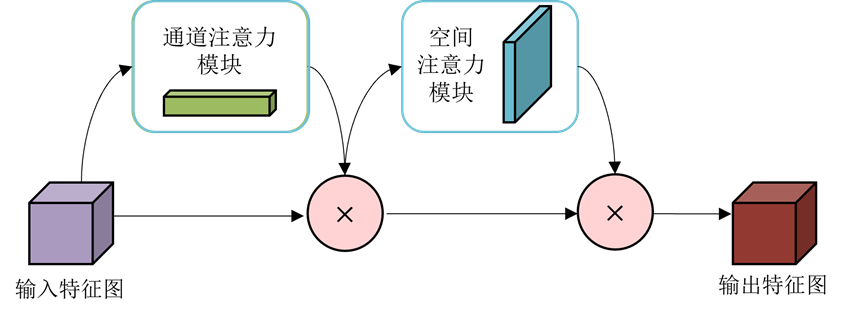
\includegraphics[width=2.5in]{./picture/CBAM结构图.png}
  \caption{CBAM结构图}
  \label{fig:CBAM}
\end{figure}

对于输入特征图$X\in R^{c\times h\times w}$ ,CBAM先使用通道注意力模块,在宽高维度上对输入进行平均池化和最大池化的操作,得到两个$c\times1\times1$大小的张量。然后,将两个张量分别经过共享卷积层,将输出进行逐元素相加,再经过非线性激活操作,得到通道注意力权值,即大小为$c\times1\times1$的张量。将该权值与输入特征图进行逐元素相乘,得到通道注意力模块的输出特征图$X^{\prime}\in R^{c\times h\times w}$ 。接着,对于通道注意力模块的输出特征图,在通道维度上进行平均池化和最大池化操作,得到两个$1\times h\times w$大小的张量。然后,将两个张量在通道维度上进行拼接,并经过一个卷积操作,将通道维度降为1。最终,经过非线性激活操作,得到空间注意力权值,即大小为$1\times h\times w$的张量。将该权值与通道注意力模块的输出特征图进行逐元素相乘,便得到经过卷积注意力模块处理后的输出特征图。根据论文[1]中的实验结果,在不同的图像分类和目标检测数据集上,将CBAM集成到不同的神经网络模型中后,模型的性能得到很大的提高,这证明了该模块的有效性。

针对YOLOv8n网络,本文将卷积注意力CBAM模块应用在了特征金字塔网络下采样过程中的每一个跨阶段局部模块之后,对不同层次的特征进行融合的Neck部分,模型框架修改后如图\ref{fig:Neck}所示。

\begin{figure}
  \centering
  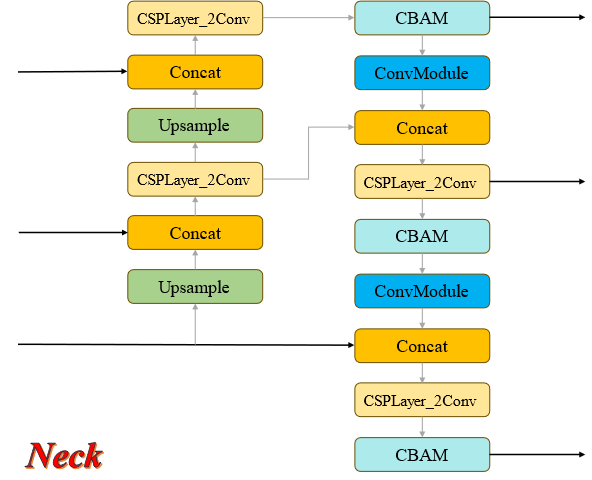
\includegraphics[width=2.5in]{./picture/应用CBAM卷积注意力模块网络Neck部分结构图.png}
  \caption{应用CBAM卷积注意力模块网络Neck部分结构图.png}
  \label{fig:Neck}
\end{figure}

%4.2 
\subsection{Transformer Block}
Transformer\cite{ref2}是一种专为处理序列数据而设计的深度学习架构。该模型利用自注意力机制实现了高效的并行计算,并具备捕获长距离依赖关系的能力。

\begin{figure}
  \centering
  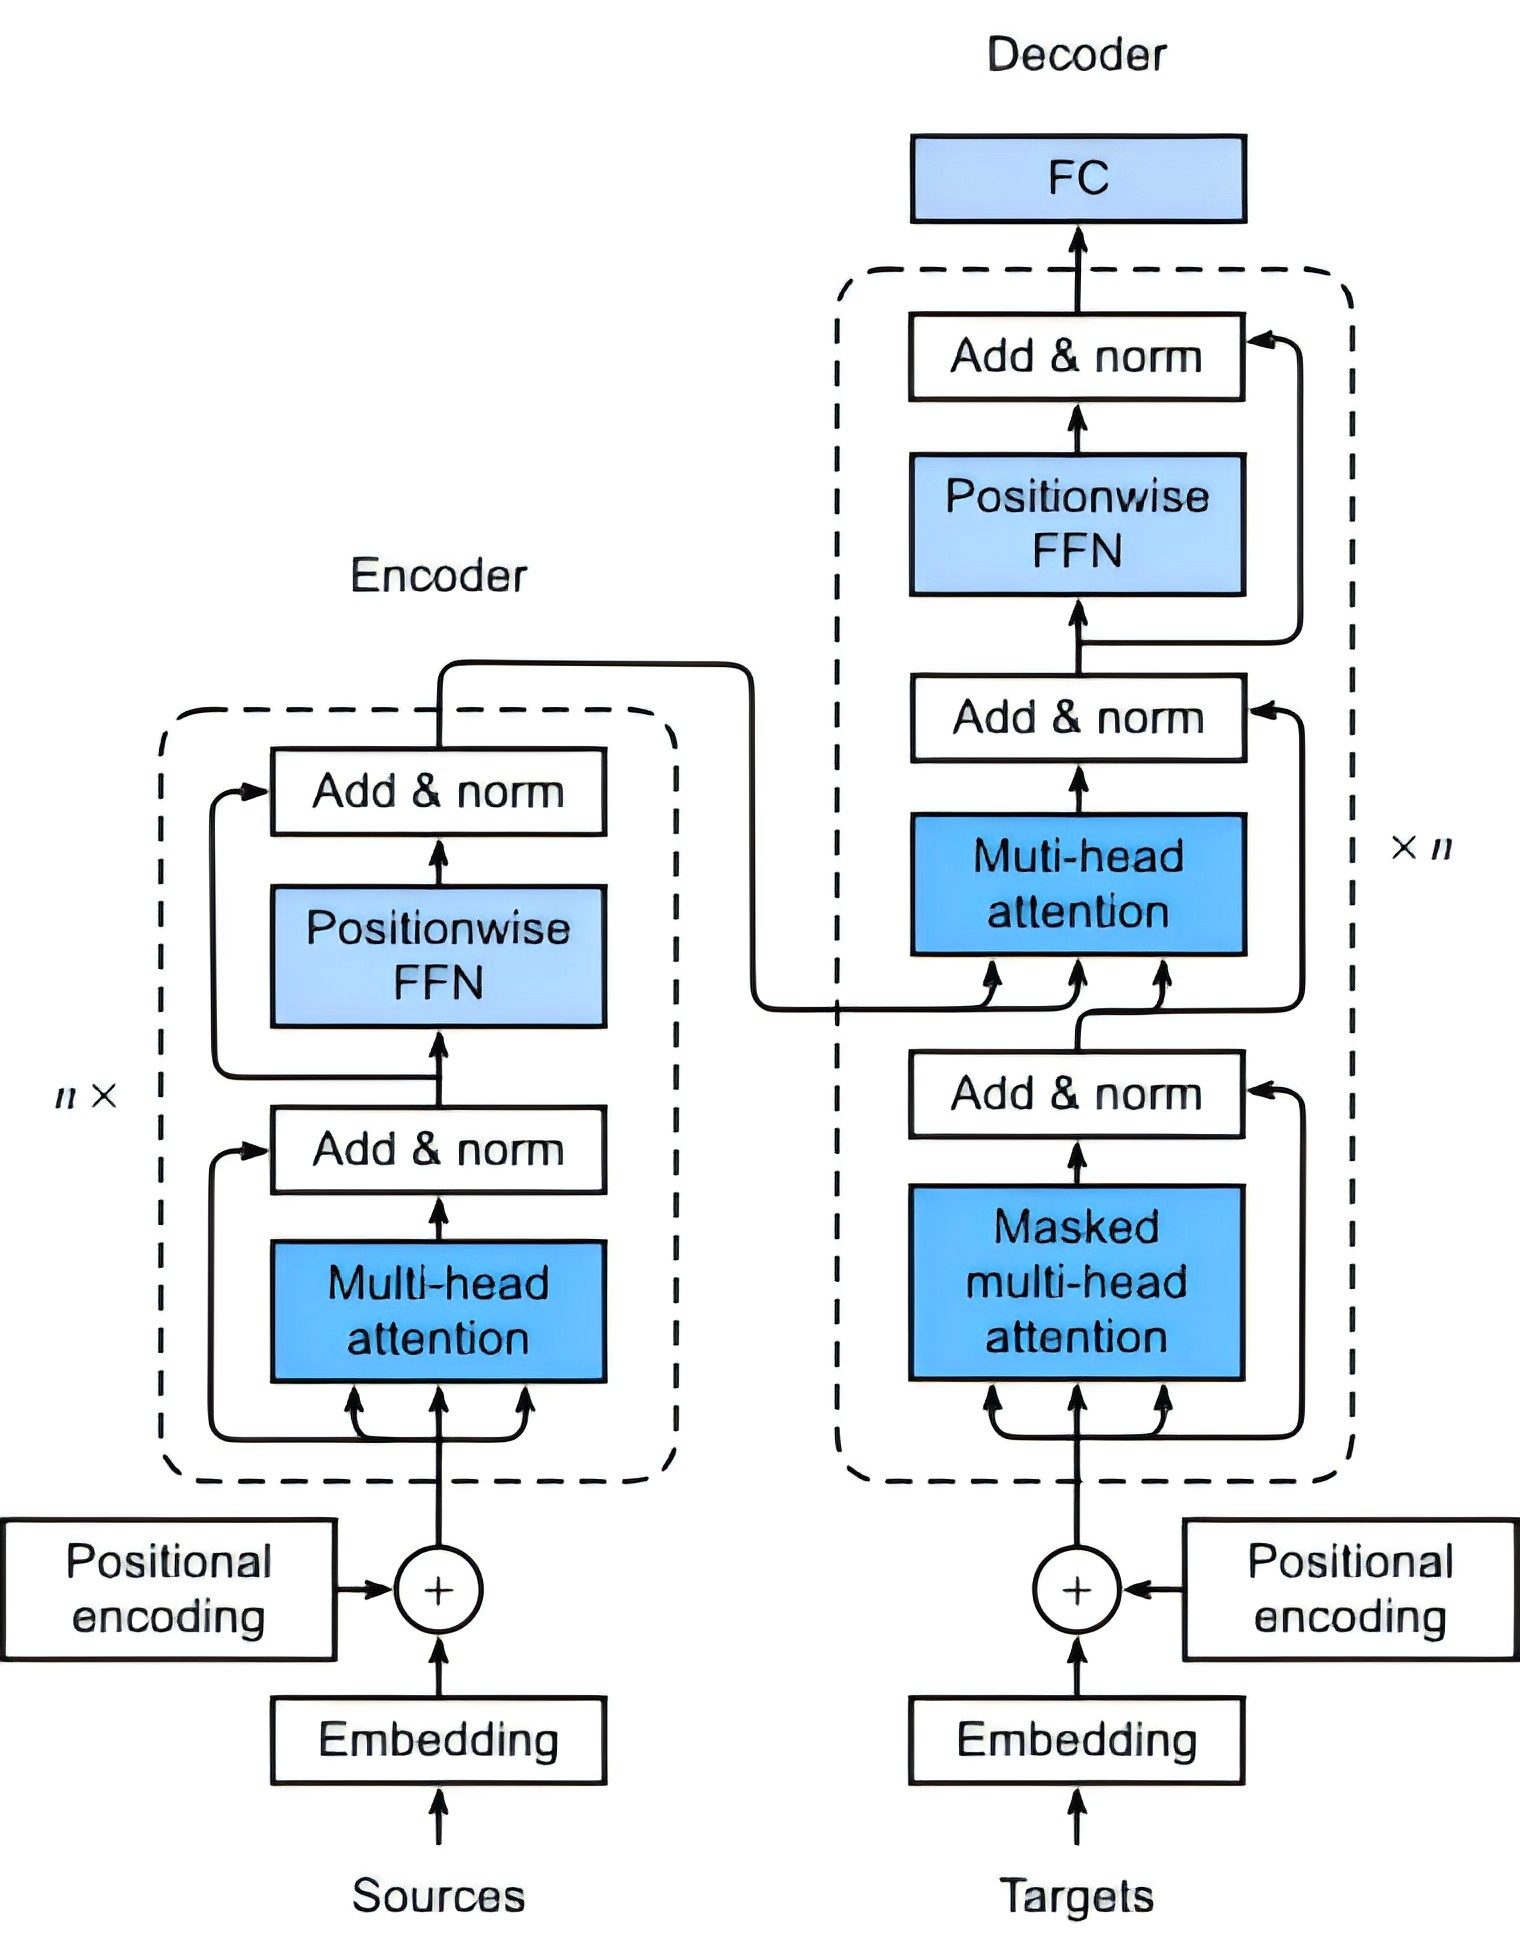
\includegraphics[width=2.5in]{./picture/transformer.jpg}
  \caption{Transformer结构图}
  \label{fig:Transformer}
\end{figure}

Transformer的结构如图\ref{fig:Transformer}所示,主要由编码器和解码器两大部分构成。编码器负责将输入信息映射为中间的隐藏状态表示,而解码器则将这些隐藏状态转换为最终的输出序列。编码器由若干相同的编码器层堆叠而成,每一层均包含自注意力机制和前馈神经网络。解码器在结构上与编码器相似,但额外增加了一个注意力层,该层用于关注编码器的输出。


多头自注意力机制是Transformer的核心,它使得模型在处理输入序列时能够同时关注序列中不同位置的信息。查询、键和值通过不同的线性变换分成多组(头),然后对每组进行自注意力计算,最后将所有头的输出拼接起来,再次通过一个线性层得到最终的输出。

前馈网络是注意力机制之后的一个关键组件。对注意力层的输出进行进一步的非线性变换,以捕获更复杂的特征和表示。

\begin{figure}
  \centering
  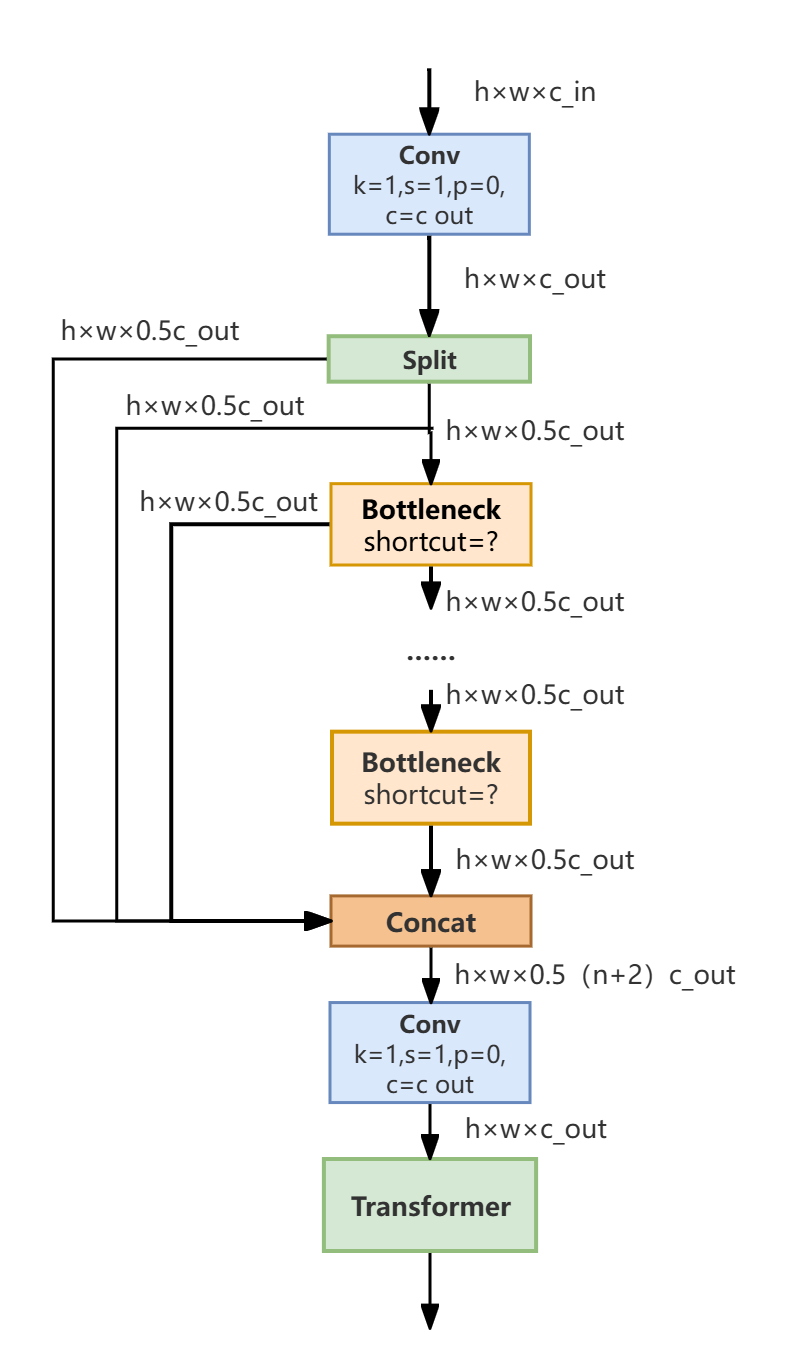
\includegraphics[width=2.5in]{./picture/C2f.png}
  \caption{添加Transformer后的C2f结构图}
  \label{fig:C2fr}
\end{figure}

针对YOLOv8n网络,本文在特征处理的中间层C2f中加入Transformer模块,修改后的C2f结构如图\ref{fig:C2fr}所示。通过引入自注意力机制,修改后的模型能够更好地捕捉长距离依赖关系,这有助于模型在处理图像时能够更好地理解全局上下文信息,从而提升特征的表示能力。且由于Transformer block能够有效捕捉全局信息,从而帮助模型在不同的尺度上捕捉到小目标的特征,能够更好地区分头盔与复杂的背景。此外,在YOLOv8n的架构中,特征融合是一个关键环节。Transformer block可以作为一种有效的特征融合工具,通过自注意力机制融合不同层次的特征信息,提高模型在各种环境下的鲁棒性,减少误报和漏报,进一步提升检测性能。




%5 实验结果
\section{实验结果}
The conclusion goes here.

%6 总结与展望
\section{总结与展望}
The conclusion goes here.

% if have a single appendix:
%\appendix[Proof of the Zonklar Equations]
% or
%\appendix  % for no appendix heading
% do not use \section anymore after \appendix, only \section*
% is possibly needed

% use appendices with more than one appendix
% then use \section to start each appendix
% you must declare a \section before using any
% \subsection or using \label (\appendices by itself
% starts a section numbered zero.)
%

% use section* for acknowledgment
\section*{致谢}


The authors would like to thank...


% Can use something like this to put references on a page
% by themselves when using endfloat and the captionsoff option.
\ifCLASSOPTIONcaptionsoff
  \newpage
\fi



% 参考文献
\begin{thebibliography}{1}

\bibitem{ref1}
	Woo S, Park J, Lee J Y, et al. CBAM: Convolutional block attention module[C]//Proceedings of the European conference on computer vision (ECCV). 2018: 3-19.

\bibitem{ref2}
Vaswani A. Attention is all you need[J]. Advances in Neural Information Processing Systems, 2017.

\end{thebibliography}


% that's all folks
\end{document}


